\chapter{Introduction to XBee}

One of the main characteristics of WSNs is the ability each node has to wirelessly communicate with other nodes. 
This is commonly performed with ZigBee compliant radios, like XBee~\cite{faludi2010bws}.

Throughout this section you will be introduced to the different components and code that will allow you to set a basic wireless network with XBee modules.

\section{The XBee module hardware configuration}\label{xbee:hardware}

Xbee modules come in different configurations. The will be using is called XBee-Series 2 with wire antenna and it is shown in Figure~\ref{fig:xbee}.

\begin{figure}[htbp]
  \centering
  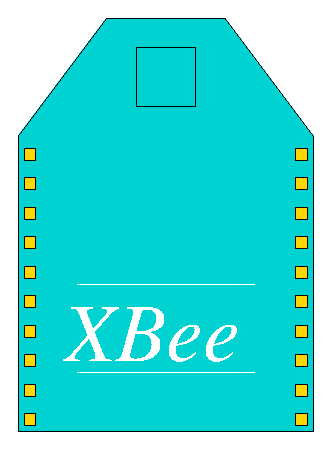
\includegraphics[width=0.7\linewidth]{figures/xbee.eps}
  \caption{XBee Series 2 with wire antenna
  \label{fig:xbee}}
\end{figure}